%%%%%%%%%%%%%%%%%%%%%%%%%%%%%%%%%%%%%%%%%%%%%%%%%%%%%%%%%%%%%%%%%%%%%%%%%%%%%%%%%%%%%%%%%%%%%%%%%%%%%%%%%%%%%%%%%%%%%%%%
%%%%%%%%%%%%%%%%%%%%%%%%%%%%%%%%%%%%%%%%%%%%%%%%%%                %%%%%%%%%%%%%%%%%%%%%%%%%%%%%%%%%%%%%%%%%%%%%%%%%%%%%%
%%%%%%%%%%%%%%%%%%%%%%%%%%%%%%%%%%%%%%%%%%%%%%%%%%   Prealamble   %%%%%%%%%%%%%%%%%%%%%%%%%%%%%%%%%%%%%%%%%%%%%%%%%%%%%%
%%%%%%%%%%%%%%%%%%%%%%%%%%%%%%%%%%%%%%%%%%%%%%%%%%                %%%%%%%%%%%%%%%%%%%%%%%%%%%%%%%%%%%%%%%%%%%%%%%%%%%%%%
%%%%%%%%%%%%%%%%%%%%%%%%%%%%%%%%%%%%%%%%%%%%%%%%%%%%%%%%%%%%%%%%%%%%%%%%%%%%%%%%%%%%%%%%%%%%%%%%%%%%%%%%%%%%%%%%%%%%%%%%


\documentclass{article}%           autres choix : report, book

\usepackage[utf8]{inputenc}
\usepackage[english]{babel}
\usepackage[T1]{fontenc}
\usepackage{textcomp}%             caractères additionnels
\usepackage{amsmath}%              pour les maths
\usepackage{amsthm}%               pour les preuves
\usepackage{amssymb}%              pour les polices maths
\usepackage{amsfonts}%             pour les polices maths
\usepackage{lmodern}%              remplacer éventuellement par txfonts, fourier, etc.
%\usepackage{xunicode}

\usepackage[a4paper]{geometry}%   taille correcte du papier

\usepackage{graphicx}%             pour inclure des images
\usepackage{xcolor}%               pour gérer les couleurs
%\usepackage{microtype}%            améliorations typographiques que du pdflatex

\usepackage{listings}%             pour faire des listings de code
\usepackage{array}%                pour faire des tableaux
\newcolumntype{L}{>{\labelitemi~~}l<{}}% Using bulltes like itemize in tabular
\usepackage{tabularx}%
\usepackage{longtable}%
\usepackage{tikz}%                 pour faire des dessins avec tikzpicture
\usetikzlibrary{arrows,shapes,backgrounds,fit}
\usepackage{tocloft}%              utiliser pour mettre des points dans la table des matières pour les sections
\usepackage{verbatim}%             


%\setlength{\parindent}{0pt}%      pour enlever les indentation en début de paragraphe
%\overfullrule=1mm%

% Macro qui donne la largeur maximale a un graphic sans violer les bordures de LaTeX
\makeatletter%
\def\maxwidth{%
	\ifdim\Gin@nat@width>\linewidth%
	\linewidth%
	\else%
	\Gin@nat@width%
	\fi%
}%
\makeatother%

%%% Fancy header and footer %%%
\usepackage{fancyhdr}%
\pagestyle{fancy}%
\usepackage{lastpage}%

%%%%%%%%%%%%%%%%%%%%%%%%%%%%%%%%%%%%%%%%%%%%%%%%%%%%%%%
%%%%%%%%%%%%%%%%%%%% Variables %%%%%%%%%%%%%%%%%%%%%%%%
%%%%%%%%%%%%%%%%%%%%%%%%%%%%%%%%%%%%%%%%%%%%%%%%%%%%%%%
\def\subject{Elasticsearch}%
\def\romain{Pignolet Romain}%
\def\romainR{Romain Pignolet}%
\def\mailromain{\href{mailto:romain.pignolet.pro@gmail.com}{\romain{}}}%
\def\datec{\today}%
%%%%%%%%%%%%%%%%
\title{\titreEntete{}}%
\author{\href{mailto:romain.pignolet.pro@gmail.com}{{\LARGE P}IGNOLET Romain}}%
\date{\datec{}}%
%%%%%%%%%%%%%%%%%%%%%%%%%%%%%%%%%%%%%%%%%%%%%%%%%%%%%%%
%%%%%%%%%%%%%%%%%%%% Fin Variables %%%%%%%%%%%%%%%%%%%%
%%%%%%%%%%%%%%%%%%%%%%%%%%%%%%%%%%%%%%%%%%%%%%%%%%%%%%%

\renewcommand{\headwidth}{\textwidth}%
\lhead{\subject{}}%
\rhead{Date : \datec{}}%
\renewcommand{\footrulewidth}{0.5pt}	% Ajout d'une ligne en bas de page
\lfoot{Last modification : \today}%
\cfoot{\thepage\ sur \pageref{LastPage}}%
\rfoot{\mailromain{}}%
% Fin Fancy header and footer

\makeatletter%
\def\maketitle{%
	\null
	\thispagestyle{empty}%
	\vfill
	\begin{center}\leavevmode
		\normalfont
		{\LARGE \textbf{\@title}\par}%
		\vskip 1cm
		{\Large \@author\par}%
		\vskip 1cm
		{\Large \@date\par}%
		\vskip 3cm%

	\end{center}%
	\vfill%
	\null%
	\cleardoublepage%
}
\makeatother%


%%%%%%%%%%%%%%%%%%%%%%%%%%%%%%%%%%%%%%%%%%%%%%%%%%%%%%%
%%%%%%%%%%%%%%%%%%%% lstlistings %%%%%%%%%%%%%%%%%%%%%%
%%%%%%%%%%%%%%%%%%%%%%%%%%%%%%%%%%%%%%%%%%%%%%%%%%%%%%%
\newlength{\MaxSizeOfLineNumbers}%
\settowidth{\MaxSizeOfLineNumbers}{99}% Adjust to maximum number of lines
\addtolength{\MaxSizeOfLineNumbers}{1.5ex}%

\definecolor{darkgreen}{rgb}{0.0,0.4,0.0}%
\definecolor{darkred}{rgb}{0.8,0.0,0.0}%
\definecolor{darkcyan}{RGB}{0,139,139}
\definecolor{darkmagenta}{RGB}{139,0,139}
\definecolor{orange}{RGB}{255,127,0}

\lstdefinestyle{command} {
	language=bash,%							Langage
	inputencoding=utf8,%					Encodage
	upquote=true,%							Utilise les "quotes" correctes
	frame=shadowbox,
	rulesepcolor=\color{lightgray},%
	%framesep=1.9mm,%
	%rulesep=1mm,%
	basicstyle=\ttfamily\small,%			Style des caractères
	identifierstyle=\color{black},%			Style du code
	commentstyle=\color{black}\ttfamily,%	Style des commentaires
	keywordstyle=\color{black}\ttfamily,%	Style des mots clés			
	stringstyle=\color{red},%				Style des chaînes de caractères
	xleftmargin=\parindent,%				Indente à gauche selon le texte
	tabsize=2,%								Largeur d'une tabulation
	breaklines=true,%						Retour à la ligne automatique si dépassement
	%numbers=left,%
	%firstnumber=1,%
	showstringspaces=false,%				Montre les espaces dans les chaînes de caractères
	xleftmargin=\MaxSizeOfLineNumbers,%		Declarer plus haut
	%	xleftmargin=15pt,%						x Rigth margin (used to align line numbers with text)
}

% Environnement pour les commandes
\lstnewenvironment{command} {%
	\lstset{
		style=command,
	}
}{}


\renewcommand{\cftsecleader}{\cftdotfill{\cftdotsep}}	% Met des "....." pour les sections de la table des matières

%%%%%%%%%%%%%%%%%%%%%%%%%%%%%%%%%%%%%%%%%%%%%%%%%%%%%%%
%%%%%%%%%%%%%%%%%%%%%%% caption %%%%%%%%%%%%%%%%%%%%%%%
%%%%%%%%%%%%%%%%%%%%%%%%%%%%%%%%%%%%%%%%%%%%%%%%%%%%%%%
\usepackage{caption}%						Caption bubbles
\DeclareCaptionFont{white}{\color{white}}%
\DeclareCaptionFormat{listing}{\colorbox{darkgray}{\parbox{\dimexpr\textwidth-2\fboxsep\relax}{#1 #2#3}}}%
%\DeclareCaptionLabelFormat{listing}{\colorbox{blue}{\parbox{5cm}{#1#2}}}
%\DeclareCaptionTextFormat{listing}{\colorbox{white}{\parbox{\textwidth}{#1}}}
\captionsetup[lstlisting]{format=listing,labelfont=white,textfont=white}%
\usepackage{subcaption}%             
\usepackage{wrapfig}%
\usepackage{float}%


\usepackage{hyperref}%             gestion des hyperliens
\hypersetup{
	pdfinfo={
		Author={\romainR{}},
		Title={Elasticsearch},
		%Subject={\subject{}},
		%ModDate={201310281730}
	}
}
\hypersetup{linkcolor=red,citecolor=blue,filecolor=dullmagenta,urlcolor=darkblue}% coloured links}
\hypersetup{pdfstartview=XYZ}%     zoom par défaut
\hypersetup{pdfkeywords={linagora,elasticsearch,mongodb}}
%\hypersetup{draft=true}
\hypersetup{final=true}
%\hypersetup{unicode=true}
%\pdfminorversion{5}
%\pdfcompresslevel{9}
%\pdfobjcompresslevel{3}


%%%%%%%%%%%%%%%%%%%%%%%%%%%%%%%%%%%%%%%%%%%%%%%%%%%%%%%%%%%%%%%%%%%%%%%%%%%%%%%%%%%%%%%%%%%%%%%%%%%%%%%%%%%%%%%%%%%%%%%%
%%%%%%%%%%%%%%%%%%%%%%%%%%%%%%%%%%%%%%%%%%%%%%%%%%                %%%%%%%%%%%%%%%%%%%%%%%%%%%%%%%%%%%%%%%%%%%%%%%%%%%%%%
%%%%%%%%%%%%%%%%%%%%%%%%%%%%%%%%%%%%%%%%%%%%%%%%%% Fin Preamble   %%%%%%%%%%%%%%%%%%%%%%%%%%%%%%%%%%%%%%%%%%%%%%%%%%%%%%
%%%%%%%%%%%%%%%%%%%%%%%%%%%%%%%%%%%%%%%%%%%%%%%%%%                %%%%%%%%%%%%%%%%%%%%%%%%%%%%%%%%%%%%%%%%%%%%%%%%%%%%%%
%%%%%%%%%%%%%%%%%%%%%%%%%%%%%%%%%%%%%%%%%%%%%%%%%%%%%%%%%%%%%%%%%%%%%%%%%%%%%%%%%%%%%%%%%%%%%%%%%%%%%%%%%%%%%%%%%%%%%%%%
%%%%%%%%%%%%%%%%%%%%%%%%%%%%%%%%%%%%%%%%%%%%%%%%%%    Document    %%%%%%%%%%%%%%%%%%%%%%%%%%%%%%%%%%%%%%%%%%%%%%%%%%%%%%
%%%%%%%%%%%%%%%%%%%%%%%%%%%%%%%%%%%%%%%%%%%%%%%%%%%%%%%%%%%%%%%%%%%%%%%%%%%%%%%%%%%%%%%%%%%%%%%%%%%%%%%%%%%%%%%%%%%%%%%%
%
\begin{document}%
%
%\maketitle%
\tableofcontents%
%
%
%
%
\newpage%



%%%%%%%%%%%%%%%%%%%%%%%%%%%%%%%%%%%%%%%%%%%%%%%%%%%%%%%%%%%%%%%%%%%%%%%%%%%%%%%%%%%%%%%%%%%%%%%%%%%%%%%%%%%%%%%%%%%%%%%%
%%%%%%%%%%%%%%%%%%%%%%%%%%%%%%%%%%%%%%%%%%    What is Elasticsearch ?    %%%%%%%%%%%%%%%%%%%%%%%%%%%%%%%%%%%%%%%%%%%%%%%
%%%%%%%%%%%%%%%%%%%%%%%%%%%%%%%%%%%%%%%%%%%%%%%%%%%%%%%%%%%%%%%%%%%%%%%%%%%%%%%%%%%%%%%%%%%%%%%%%%%%%%%%%%%%%%%%%%%%%%%%
\section{What is Elasticsearch ?}

\paragraph{} Elasticsearch is a real-time distributed search and analytics engine.

\paragraph{} It is used for full text search, structured search, analytics, and all three in combination.

\subsection{Who use Elasticsearch ?}

\begin{itemize}
	\item Wikipedia uses Elasticsearch to provide full text search with highlighted search snippets, and search-as-you-type and did-you-mean suggestions.
	\item The Guardian uses Elasticsearch to combine visitor logs with social network data to provide real-time feedback to their editors about the public’s response to new articles.
	\item StackOverflow combines full text search with geolocation queries and uses more-like-this to find related questions and answers.
	\item GitHub uses Elasticsearch to query 130 billion lines of code.
	\item Goldman Sachs uses it to index 5TB of log data every day, and a number of investment banks use it purely to analyze movements in the stock market.
\end{itemize}

\subsection{Dependency}

\begin{itemize}
	\item Elasticsearch is a search engine built on top of Apache Lucene™, a full-text search engine library.
	\item Elasticsearch is write in Java so you need the JVM.
\end{itemize}

\subsection{Features}

Elasticsearch is:
\begin{itemize}
	\item a distributed real-time document store where \textbf{every field} is indexed and searchable
	\item a distributed search engine with real-time analytics
	\item capable of scaling to hundreds of servers and petabytes of structured and unstructured data.
\end{itemize}

%%%%%%%%%%%%%%%%%%%%%%%%%%%%%%%%%%%%%%%%%%%%%%%%%%%%%%%%%%%%%%%%%%%%%%%%%%%%%%%%%%%%%%%%%%%%%%%%%%%%%%%%%%%%%%%%%%%%%%%%
%%%%%%%%%%%%%%%%%%%%%%%%%%%%%%%%%%%%%%    Installation and simple example    %%%%%%%%%%%%%%%%%%%%%%%%%%%%%%%%%%%%%%%%%%%
%%%%%%%%%%%%%%%%%%%%%%%%%%%%%%%%%%%%%%%%%%%%%%%%%%%%%%%%%%%%%%%%%%%%%%%%%%%%%%%%%%%%%%%%%%%%%%%%%%%%%%%%%%%%%%%%%%%%%%%%
\section{Installation and simples examples}

\subsection{Installation}

Simply download the archive on the officiel website and decompress.

\subsection{Elasticsearch hierarchy}

The Elasticsearch folder contains:

\begin{itemize}
	\item bin : launching scripts
	\item config : configuration files
	\item data : database location
	\item lib : library dependency
	\item logs : logs location
	\item plugins : plugins location
\end{itemize}

\subsection{Launching Elasticsearch}

Simply run this command:
\begin{command}
./bin/elasticsearch
\end{command}

Test it out by running this command:
\begin{command}
curl 'http://localhost:9200/?pretty'
\end{command}

You should see a response like this:
\begin{command}
{
	"status" : 200,
	"name" : "Brother Nature",
	"version" : {
		"number" : "1.1.0",
		"build_hash" : "2181e113dea80b4a9e31e58e9686658a2d46e363",
		"build_timestamp" : "2014-03-25T15:59:51Z",
		"build_snapshot" : false,
		"lucene_version" : "4.7"
	},
	"tagline" : "You Know, for Search"
}
\end{command}

\subsection{Communicate with Elasticsearch}

There are two ways to communicate with Elasticsearch:
\begin{itemize}
	\item Java API over port 9300
	\item Restful API with JSON over port 9200
\end{itemize}

Hereinafter we will discuss only about the Restful API.

\subsection{How documents are stored ?}

\paragraph{} Elasticsearch is document oriented, meaning that it stores entire objects or documents. Not only does it store them, it also indexes the contents of each document in order to make them searchable.

\paragraph{} In Elasticsearch, a document belongs to a type, and those types live inside an index. Some parallels to a traditional relational database:

\begin{tabular}{|c|c|c|c|c|}
\hline
\textbf{Relational DB} & Databases & Tables & Rows & Columns\\
\hline
\textbf{Mongo DB} & Databases & Collections & Documents & Fields\\
\hline
\textbf{Elasticsearch} & Indices/Indexes & Types & Documents & Fields\\
\hline
\end{tabular}

%%%%%%%%%%%%%%%%%%%%%%%%%%%%%%%%%%%%%%%%%%%%%%%%%%%%%%%%%%%%%%%%%%%%%%%%%%%%%%%%%%%%%%%%%%%%%%%%%%%%%%%%%%%%%%%%%%%%%%%%
%%%%%%%%%%%%%%%%%%%%%%%%%%%%%%%%%%%%%%%%%%%%%%%%    Restful API    %%%%%%%%%%%%%%%%%%%%%%%%%%%%%%%%%%%%%%%%%%%%%%%%%%%%%
%%%%%%%%%%%%%%%%%%%%%%%%%%%%%%%%%%%%%%%%%%%%%%%%%%%%%%%%%%%%%%%%%%%%%%%%%%%%%%%%%%%%%%%%%%%%%%%%%%%%%%%%%%%%%%%%%%%%%%%%
\section{Restful API}

Behavior depending on the query type:
\begin{itemize}
	\item PUT : create or update a document
	\item GET : retrieve document
	\item HEAD : check if a document exists
	\item DELETE : delete a document
\end{itemize}

Elasticsearch returns an HTTP status code like 200 OK and (except for HEAD requests) a JSON encoded response body.

\subsection{PUT Request}

\paragraph{Syntax}:

\begin{command}
curl -XPUT 'http://<hostname>:9200/<index>/<type>/[<id>]' -d '
{
    ...
}'
\end{command}

\begin{itemize}
	\item <hostname> : the hostname where Elasticsearch is running
	\item <index> : the index name
	\item <type> : the type name
	\item <id> : the ID of this particular object. If omited, the ID will be generated automatically.
\end{itemize}

If the operation succeed, the result of the above PUT operation is like:

\begin{command}
{
	"_index" : <index>,
	"_type" : <type>,
	"_id" : <id>,
	"_version" : [1..9.2e+18],
	"created" : true|false
}
\end{command}

\begin{itemize}
	\item \_version : Each indexed document is given a version number. By default, internal versioning is used that starts at 1 and increments with each update, deletes included.
	\item created : true if the PUT request create a new document, false if the PUT request update a existing document. Note : if the PUT request is execute without specifying <id> then the created field will be true.
\end{itemize}

\paragraph{Example}:

We want to save three documents of type employee and are in the megacorp.

\begin{command}
curl -XPUT 'localhost:9200/megacorp/employee/1' -d '
{
	"first_name" : "John",
	"last_name"  : "Smith",
	"age"        : 25,
	"about"      : "I love to go rock climbing",
	"interests"  : [ "sports", "music" ]
}'
curl -XPUT 'localhost:9200/megacorp/employee/2' -d '
{
	"first_name" : "Douglas",
	"last_name"  : "Fir",
	"age"        : 35,
	"about"      : "I like to build cabinets",
	"interests"  : [ "forestry" ]
}'
curl -XPUT 'localhost:9200/megacorp/employee/3' -d '
{
	"first_name" : "Jane",
	"last_name"  : "Smith",
	"age"        : 32,
	"about"      : "I like to collect rock albums",
	"interests"  : [ "music" ]
}'
\end{command}


\subsection{GET Request}

\paragraph{Syntax}:

\begin{command}
curl -XGET 'http://<hostname>:9200/<index>/<type>/<id>[/_<endpoint>][?<option1>=<value1>[&<optionN>=<valueN>...]]'
\end{command}

\begin{itemize}
	\item <hostname> : the hostname where Elasticsearch is running
	\item <index> : the index name
	\item <type> : the type name. Set it to \texttt{\_all} in order to fetch the first document matching the id across all types.
	\item <id> : the ID of this particular object.
\end{itemize}

If the operation succeed, the result of the above GET operation is like:

\begin{command}
{
	"_index" : <index>,
	"_type" : <type>,
	"_id" : <id>,
	"_version" : [1..9.2e+18],
	"found": true|false,
	"_source" : {
		...
	}
}
\end{command}

\begin{itemize}
	\item found : if the GET request found at least one match then \texttt{found} is true
	\item \_source : the document content only if \texttt{found} is true
\end{itemize}

\paragraph{Example}:

\begin{command}
curl -XGET 'localhost:9200/megacorp/employee/2?pretty'
\end{command}

\begin{command}
{
	"_index" : "megacorp",
	"_type" : "employee",
	"_id" : "2",
	"_version" : 1,
	"found": true,
	"_source" : {
		"first_name" : "Douglas",
		"last_name"  : "Fir",
		"age"        : 35,
		"about"      : "I like to build cabinets",
		"interests"  : [ "forestry" ]
	}
}
\end{command}

\subsubsection{Endpoint \_source}

To get just the \texttt{\_source} field of the document, without any additional content around it.

\begin{command}
curl -XGET 'http://localhost:9200/megacorp/employee/1/_source?pretty'
\end{command}

\begin{command}
{
	"first_name" : "John",
	"last_name"  : "Smith",
	"age"        : 25,
	"about"      : "I love to go rock climbing",
	"interests"  : [ "sports", "music" ]
}
\end{command}

\subsubsection{Endpoint \_search}

We will search for all employees, with this request:
\begin{command}
curl -XGET 'localhost:9200/megacorp/employee/_search?pretty'
\end{command}

By default, a search will return the top 10 results in the \texttt{hits} array.

\begin{command}
{
	"took" : 3,
	"timed_out" : false,
	"_shards" : {
		"total" : 5,
		"successful" : 5,
		"failed" : 0
	},
	"hits" : {
		"total" : 3,
		"max_score" : 1.0,
		"hits" : [ {
 			"_index" : "megacorp",
 			"_type" : "employee",
 			"_id" : "3",
 			"_score" : 1.0,
 			"_source" : {
				"first_name" : "Jane",
				"last_name"  : "Smith",
				"age"        : 32,
				"about"      : "I like to collect rock albums",
				"interests"  : [ "music" ]
			}
		}, {
			"_index" : "megacorp",
			"_type" : "employee",
			"_id" : "1",
			"_score" : 1.0,
			"_source" : {
				"first_name" : "John",
				"last_name"  : "Smith",
				"age"        : 25,
				"about"      : "I love to go rock climbing",
				"interests"  : [ "sports", "music" ]
			}
		}, {
			"_index" : "megacorp",
			"_type" : "employee",
			"_id" : "2",
			"_score" : 1.0,
			"_source" : {
				"first_name" : "Douglas",
				"last_name"  : "Fir",
				"age"        : 35,
				"about"      : "I like to build cabinets",
				"interests"  : [ "forestry" ]
			}
		}
	] }
}
\end{command}

Note : search includes the whole document itself in the \texttt{\_source} field.

\subsubsection{Endpoint \_search with query option}

You can use the query option (\texttt{q}) to specify a simple query like:

\begin{command}
curl -XGET 'localhost:9200/megacorp/employee/_search?q=last_name:Smith&pretty'
\end{command}

This query will get all employee where \texttt{last\_name} field is equal to "Smith".

\begin{command}
{
	"took" : 73,
	"timed_out" : false,
	"_shards" : {
		"total" : 5,
		"successful" : 5,
		"failed" : 0
	},
	"hits" : {
		"total" : 2,
		"max_score" : 0.30685282,
		"hits" : [ {
			"_index" : "megacorp",
			"_type" : "employee",
			"_id" : "3",
			"_score" : 0.30685282,
			"_source" : {
				"first_name" : "Jane",
				"last_name"  : "Smith",
				"age"        : 32,
				"about"      : "I like to collect rock albums",
				"interests"  : [ "music" ]
			}
		}, {
			"_index" : "megacorp",
			"_type" : "employee",
			"_id" : "1",
			"_score" : 0.30685282,
			"_source" : {
				"first_name" : "John",
				"last_name"  : "Smith",
				"age"        : 25,
				"about"      : "I love to go rock climbing",
				"interests"  : [ "sports", "music" ]
			}
		} ]
	}
}
\end{command}

\subsubsection{Endpoint \_search with \textit{Query DSL}}

This query use \textit{Query DSL} to do the same query as before : find all employee where last name is Smith.

\begin{command}
curl -XGET 'localhost:9200/megacorp/employee/_search?pretty' -d '
{
	"query" : {
		"match" : {
			"last_name" : "smith"
		}
	}
}'
\end{command}

Now we will use a filter to find all employee where last name is Smith and age greater than 30.

\begin{command}
curl -XGET 'localhost:9200/megacorp/employee/_search?pretty' -d '
{
	"query" : {
		"filtered" : {
			"filter" : {
				"range" : {
					"age" : { "gt" : 30 }
				}
			},
			"query" : {
				"match" : {
					"last_name" : "smith" 
				}
			}
		}
	}
}'
\end{command}

We use a range filter with a query.

\begin{command}
{
	"took" : 13,
	"timed_out" : false,
	"_shards" : {
		"total" : 5,
		"successful" : 5,
		"failed" : 0
	},
	"hits" : {
		"total" : 1,
		"max_score" : 0.30685282,
		"hits" : [ {
			"_index" : "megacorp",
			"_type" : "employee",
			"_id" : "3",
			"_score" : 0.30685282,
			"_source" : {
				"first_name" : "Jane",
				"last_name"  : "Smith",
				"age"        : 32,
				"about"      : "I like to collect rock albums",
				"interests"  : [ "music" ]
			}
		} ]
	}
}
\end{command}

\paragraph{Full text search}:

We want to find all employee where \texttt{about} field contains "rock" and/or "climbing".

\begin{command}
curl -XGET 'localhost:9200/megacorp/employee/_search?pretty' -d '
{
    "query" : {
        "match" : {
            "about" : "rock climbing"
        }
    }
}'
\end{command}

\begin{command}
{
	"took" : 8,
	"timed_out" : false,
	"_shards" : {
		"total" : 5,
		"successful" : 5,
		"failed" : 0
	},
	"hits" : {
		"total" : 2,
		"max_score" : 0.16273327,
		"hits" : [ {
			"_index" : "megacorp",
			"_type" : "employee",
			"_id" : "1",
			"_score" : 0.16273327,
			"_source" : {
				"first_name" : "John",
				"last_name"  : "Smith",
				"age"        : 25,
				"about"      : "I love to go rock climbing",
				"interests"  : [ "sports", "music" ]
			}
		}, {
			"_index" : "megacorp",
			"_type" : "employee",
			"_id" : "3",
			"_score" : 0.016878016,
			"_source" : {
				"first_name" : "Jane",
				"last_name"  : "Smith",
				"age"        : 32,
				"about"      : "I like to collect rock albums",
				"interests"  : [ "music" ]
			}
		} ]
	}
}
\end{command}

\paragraph{} By default, Elasticsearch sorts matching results by their relevance score, that is: by how well each document matched the query. The first and highest scoring result is obvious: John Smith’s \texttt{about} field clearly says "rock climbing" in it.

\paragraph{} But why did Jane Smith, come back as a result? The reason her document was returned is because the word "rock" was mentioned in her \texttt{about} field. Because only "rock" was mentioned, and not "climbing", her \texttt{\_score} is lower than John’s.

\paragraph{Phrase search}:

But now we want "rock" \textbf{and} "climbing".

\begin{command}
curl -XGET 'localhost:9200/megacorp/employee/_search?pretty' -d '
{
    "query" : {
        "match_phrase" : {
            "about" : "rock climbing"
        }
    }
}'
\end{command}

\begin{command}
{
	"took" : 9,
	"timed_out" : false,
	"_shards" : {
		"total" : 5,
		"successful" : 5,
		"failed" : 0
	},
	"hits" : {
		"total" : 1,
		"max_score" : 0.23013961,
		"hits" : [ {
			"_index" : "megacorp",
			"_type" : "employee",
			"_id" : "1",
			"_score" : 0.23013961,
			"_source" : {
				"first_name" : "John",
				"last_name"  : "Smith",
				"age"        : 25,
				"about"      : "I love to go rock climbing",
				"interests"  : [ "sports", "music" ]
			}
		} ]
	}
}
\end{command}

Only "John" match the query.

\paragraph{Highlight search}:

Now we want to see : "Why the document matched the query ?" so we use the \texttt{highlight} parameter.

\begin{command}
curl -XGET 'localhost:9200/megacorp/employee/_search?pretty' -d '
{
	"query" : {
		"match_phrase" : {
			"about" : "rock climbing"
		}
	},
	"highlight": {
		"fields" : {
			"about" : {}
		}
	}
}'
\end{command}

\begin{command}
{
	"took" : 64,
	"timed_out" : false,
	"_shards" : {
		"total" : 5,
		"successful" : 5,
		"failed" : 0
	},
	"hits" : {
		"total" : 1,
		"max_score" : 0.23013961,
		"hits" : [ {
			"_index" : "megacorp",
			"_type" : "employee",
			"_id" : "1",
			"_score" : 0.23013961,
			"_source" : {
				"first_name" : "John",
				"last_name"  : "Smith",
				"age"        : 25,
				"about"      : "I love to go rock climbing",
				"interests"  : [ "sports", "music" ]
			},
			"highlight" : {
				"about" : [ "I love to go <em>rock</em> <em>climbing</em>" ]
			}
		} ]
	}
}
\end{command}

As you can see, the matched words are between \texttt{<em>} HTML tags.

\subsubsection{Option fields (deprecated since 1.0.0, use \texttt{\_source} option instead)}

The get operation allows specifying a set of stored fields that will be returned by passing the fields parameter.

\begin{command}
curl -XGET 'http://localhost:9200/megacorp/employee/1?fields=last_name,about&pretty'
\end{command}

We will get the employee with \texttt{id} is equal to 1 and show only the field \texttt{last\_name} and \texttt{about}.

\begin{command}
{
	"_index" : "megacorp",
	"_type" : "employee",
	"_id" : "1",
	"_version" : 1,
	"found" : true,
	"fields" : {
		"about" : [ "I love to go rock climbing" ],
		"last_name" : [ "Smith" ]
	}
}
\end{command}

\subsubsection{Option \_source}

By default, the get operation returns the contents of the \texttt{\_source} field unless you have used the \texttt{fields} parameter or if the \texttt{\_source} field is disabled. You can turn off \texttt{\_source} retrieval by using the \texttt{\_source} parameter:

\begin{command}
curl -XGET 'http://localhost:9200/megacorp/employee/1?_source=false&pretty'
\end{command}

\begin{command}
{
	"_index" : "megacorp",
	"_type" : "employee",
	"_id" : "1",
	"_version" : 1,
	"found" : true
}
\end{command}

If you want specific fields, you can list it with \texttt{\_source} option like:

\begin{command}
curl -XGET 'http://localhost:9200/megacorp/employee/1?_source=last_name,about&pretty'
\end{command}

\begin{command}
{
	"_index" : "megacorp",
	"_type" : "employee",
	"_id" : "1",
	"_version" : 1,
	"found" : true,
	"_source" : {
		"about" : "I love to go rock climbing",
		"last_name" : "Smith"
	}
}
\end{command}

\subsubsection{Option \_source\_include and \_source\_exclude}

If you only need one or two fields from the complete \texttt{\_source}, you can use the \texttt{\_source\_include} \& \texttt{\_source\_exclude} parameters to include or filter out that parts you need. This can be especially helpful with large documents where partial retrieval can save on network overhead. Both parameters take a comma separated list of fields or wildcard expressions.

% \begin{command}
% curl -XGET 'http://localhost:9200/megacorp/employee/1?_source_include=*_name&_source_exclude=about&pretty'
% \end{command}

\subsubsection{Endpoint \_mget}

\paragraph{} Combining multiple requests into one avoids the network overhead of processing each request individually. If you know that you need to retrieve multiple documents from Elasticsearch, it is faster to retrieve them all in a single request using the \textit{multi-get} or \texttt{mget} API, instead of document-by-document.

\paragraph{} The \texttt{mget} API expects a \texttt{docs} array, each element of which specifies the \texttt{\_index}, \texttt{\_type} and \texttt{\_id} metadata of the document you wish to retrieve. You can also specify a \texttt{\_source} parameter if you just want to retrieve one or more specific fields:

\begin{command}
curl -XGET 'http://localhost:9200/_mget?pretty' -d '
{
	"docs" : [
		{
			"_index" : "megacorp",
			"_type" :  "employee",
			"_id" :    1
		},
		{
			"_index" : "megacorp",
			"_type" :  "employee",
			"_id" :    2,
			"_source": [ "about" , "last_name" ]
		},
		{
			"_index" : "megacorp",
			"_type" :  "employee",
			"_id" :    3,
			"_source": "first_name"
		}
	]
}'
\end{command}

\begin{command}
{
	"docs" : [ {
		"_index" : "megacorp",
		"_type" : "employee",
		"_id" : "1",
		"_version" : 1,
		"found" : true,
		"_source" : {
			"first_name" : "John",
			"last_name"  : "Smith",
			"age"        : 25,
			"about"      : "I love to go rock climbing",
			"interests"  : [ "sports", "music" ]
		}
	}, {
		"_index" : "megacorp",
		"_type" : "employee",
		"_id" : "2",
		"_version" : 1,
		"found" : true,
		"_source" : {
			"about":"I like to build cabinets",
			"last_name":"Fir"
		}
	}, {
		"_index" : "megacorp",
		"_type" : "employee",
		"_id" : "3",
		"_version" : 1,
		"found" : true,
		"_source" : {
			"first_name":"Jane"
		}
  } ]
}
\end{command}

You can specify a default \texttt{/\_index} or a default \texttt{/\_index/\_type} in the URL. The following request return the same results as previous request:

\begin{command}
curl -XGET 'http://localhost:9200/megacorp/employee/_mget?pretty' -d '
{
	"docs" : [
		{
			"_id" : 1
		},
		{
			"_id" : 2,
			"_source": [ "about" , "last_name" ]
		},
		{
			"_id" : 3,
			"_source": "first_name"
		}
	]
}'
\end{command}

If all the documents have the same \texttt{\_index} and \texttt{\_type}, then you can just pass an array of \texttt{ids} instead of the full \texttt{docs} array:

\begin{command}
curl -XGET 'http://localhost:9200/megacorp/employee/_mget?pretty' -d '
{
	"ids" : [ "2", "1" ]
}'
\end{command}

\subsubsection{Endpoint \_explain}

\paragraph{} You can use the \texttt{explain} API to understand why one particular document matched or, more importantly, why it \textbf{didn’t match}.

\paragraph{} The path for the request is \texttt{/<index>/<type>/<id>/\_explain}, as in:

\begin{command}
curl -XGET 'localhost:9200/megacorp/employee/1/_explain?pretty' -d '
{
	"query" : {
		"match" : {
			"last_name" : "smit" 
		}
	}
}'
\end{command}

Same query but with \texttt{q} option :
\begin{command}
curl -XGET 'localhost:9200/megacorp/employee/1/_explain?q=last_name:smit&pretty'
\end{command}

\begin{command}
{
	"_index" : "megacorp",
	"_type" : "employee",
	"_id" : "1",
	"matched" : false,
	"explanation" : {
		"value" : 0.0,
		"description" : "no matching term"
	}
}
\end{command}

There are no matching for "smit" in the document with \texttt{\_id} is equal to 1 with type \texttt{employee} and in the \texttt{megacorp} index because "smit" is not equal to "smith". The match could be a success if we had used a wildcard expression (*) like:

\begin{command}
curl -XGET 'localhost:9200/megacorp/employee/1/_explain?q=last_name:smit*&pretty'
\end{command}

\subsection{HEAD Request}

This request check if the document exists or not. If the document exists, the HTTP header is \texttt{200 OK}, otherwise the HTTP header is \texttt{404 Not Found}.

\subsection{DELETE Request}

If you want to remove the \texttt{megacorp} index.

\begin{command}
curl -XDELETE 'http://localhost:9200/megacorp'
\end{command}


%%%%%%%%%%%%%%%%%%%%%%%%%%%%%%%%%%%%%%%%%%%%%%%%%%%%%%%%%%%%%%%%%%%%%%%%%%%%%%%%%%%%%%%%%%%%%%%%%%%%%%%%%%%%%%%%%%%%%%%%
%%%%%%%%%%%%%%%%%%%%%%%%%%%%%%%%%%%%%%%%%%%%%%    How it works ?    %%%%%%%%%%%%%%%%%%%%%%%%%%%%%%%%%%%%%%%%%%%%%%%%%%%%
%%%%%%%%%%%%%%%%%%%%%%%%%%%%%%%%%%%%%%%%%%%%%%%%%%%%%%%%%%%%%%%%%%%%%%%%%%%%%%%%%%%%%%%%%%%%%%%%%%%%%%%%%%%%%%%%%%%%%%%%
\section{How it works ?}

\subsection{Indexing (\_all field)}

\paragraph{} In Elasticsearch, \textbf{all data in every field is indexed by default}. That is, every field has a dedicated \textit{inverted index} for fast retrieval.

\paragraph{} When you index a document, Elasticsearch takes the string values of all of its fields and concatenates them into one big string which it indexes as the special \texttt{\_all} field.

\paragraph{} If you decide that you no longer need the \texttt{\_all} field, you can disable it with this mapping:

\begin{command}
curl -XPUT 'localhost:9200/<index>/_mapping/<type>/' -d '
{
    <type>: {
        "_all": { "enabled": false }
    }
}'
\end{command}

\paragraph{} Inclusion in the \texttt{\_all} field can be controlled on a field-by-field basis using the \texttt{include\_in\_all} setting, which defaults to true. Setting \texttt{include\_in\_all} on an object (or on the root object) changes the default for all fields within that object.

\begin{command}
curl -XPUT 'localhost:9200/<index>/<type>/_mapping/' -d '
{
    <type>: {
        "include_in_all": false,
        "properties": {
            "about": {
                "type": "string",
                "include_in_all": true
            },
            ...
        }
    }
}'
\end{command}

\paragraph{} You may find that you want to keep the \texttt{\_all} field around to use as a catch-all full text field just for specific fields, such as title, overview, summary, tags etc. Instead of disabling the \texttt{\_all} field completely, disable \texttt{include\_in\_all} for all fields by default, and enable it only on the fields you choose:

\subsection{Document metadata}

\begin{itemize}
	\item \_index : Where the document lives. (Like a Database in Relational DB)
	\item \_type : The class of object that the document represents. (Like a Table in Relational DB)
	\item \_id : The unique identifier for the document.
\end{itemize}

\subsection{Fields}
\label{Fields}

\paragraph{} When you sort on a field, Elasticsearch needs access to the value for that field for every document which matches the query. The inverted index, which performs very well when searching, is not the ideal structure for sorting on field values.

\begin{itemize}
	\item When searching we need to be able to map a term to a list of documents.
	\item When sorting, we need to map a document to its terms. In other words, we need to “uninvert” the inverted index. 
\end{itemize}

\paragraph{} In order to make sorting efficient, Elasticsearch loads all of the values for the field that you want to sort on into memory. This is referred to as \textit{field data}.

\paragraph{Important} It doesn’t just load the values for the documents that matched a particular query. It loads the values from every document in your index, regardless of the document type.

\paragraph{Reason} The reason that it loads all values into memory is that uninverting the index from disk is slow. Even though you may only need the values for a few docs for the current request, you will probably need access to the values for other docs on the next request, so it makes sense to load all the values into memory at once, and to keep them there.

\subsection{Types and Mappings}

\paragraph{} A type in Elasticsearch represents a class of similar documents. A type consists of a \textbf{name}  --  such as \texttt{user} or \texttt{blogpost}  --  and a \textbf{mapping}. The mapping, like a database schema, describes the fields or properties that documents of that type may have, the datatype of each field  --  \texttt{string}, \texttt{integer}, \texttt{date} etc  --  and how those fields should be indexed and stored by Lucene. So a type is like a table in relational database.


\paragraph{Lucene} A document in Lucene consists of a simple list of field-value pairs. Lucene doesn’t care if the values are strings or numbers or dates  --  all values are just treated as "opaque bytes". When we index a document in Lucene, the values for each field are added to the inverted index for the associated field.

\paragraph{Type implementation} Elasticsearch types are implemented on top of this simple foundation. An index may have several types, each with their own mapping, and documents of any of these types may be stored in the same index.

\paragraph{Sort conflicts} When two documents in the same index have different type for the same field name, will either produce unexpected results or fail outright.

\paragraph{Sort conflicts example}:

Type: user. 
\begin{command}
{ "login": "john_smith" }
\end{command}

Type: event. 
\begin{command}
{ "login": "2014-06-01" }
\end{command}
These two documents are in the same index.

\paragraph{} If we now try to sort on the \texttt{event.login} field then Elasticsearch needs to load the values in the \texttt{login} field into memory. As we said in \ref{Fields}, it loads the values for all documents in the index regardless of their type. It will either try to load these values as a string or as a date, depending on which \texttt{login} field it sees first.

\paragraph{Sort conflicts solution} To ensure that you don’t run into these conflicts, it is advisable to ensure that fields with the \textbf{same name} are mapped in the \textbf{same way} in every type in an index.

\paragraph{} To know the mapping for a type you can do a GET request with path: \texttt{/<index>/\_mapping/<type>}

\begin{command}
curl -XGET 'localhost:9200/megacorp/_mapping/employee?pretty'
\end{command}

\begin{command}
{
	"megacorp" : {
		"mappings" : {
			"employee" : {
				"properties" : {
					"about" : {
						"type" : "string"
					},
					"age" : {
						"type" : "long"
					},
					"first_name" : {
						"type" : "string"
					},
					"interests" : {
						"type" : "string"
					},
					"last_name" : {
						"type" : "string"
					}
				}
			}
		}
	}
}
\end{command}

\subsection{Relevance (scoring)}

\paragraph{} The relevance score of each document is represented by a positive floating point number called the \texttt{\_score}  --  the higher the \texttt{\_score}, the more relevant the document.

\paragraph{Understanding the score} When debugging a complex query, it can be difficult to understand exactly how a \texttt{\_score} has been calculated. Elasticsearch has the option of producing an explanation with every search result, by setting the \texttt{explain} parameter to true.

\begin{command}
curl -XGET 'localhost:9200/megacorp/employee/_search?explain&pretty'
\end{command}

\paragraph{} One of the important factors taken into account by the relevance algorithm is the length of the field: the shorter the field, the more important. A term that appears in a short \texttt{last\_name} field is likely to be more important than the same term which appears somewhere in a long \texttt{about} field. This distinction between field lengths disappears in the \texttt{\_all} field.

%%%%%%%%%%%%%%%%%%%%%%%%%%%%%%%%%%%%%%%%%%%%%%%%%%%%%%%%%%%%%%%%%%%%%%%%%%%%%%%%%%%%%%%%%%%%%%%%%%%%%%%%%%%%%%%%%%%%%%%%
%%%%%%%%%%%%%%%%%%%%%%%%%%%%%%%%%%%%%%%%%%%%%%%%%%    Cluster    %%%%%%%%%%%%%%%%%%%%%%%%%%%%%%%%%%%%%%%%%%%%%%%%%%%%%%%
%%%%%%%%%%%%%%%%%%%%%%%%%%%%%%%%%%%%%%%%%%%%%%%%%%%%%%%%%%%%%%%%%%%%%%%%%%%%%%%%%%%%%%%%%%%%%%%%%%%%%%%%%%%%%%%%%%%%%%%%
\section{Cluster}

\subsection{Definitions}

\paragraph{Node} A node is a running instance of Elasticsearch, while a cluster consists of one or more nodes with the same \texttt{cluster.name} that are working together to share their data and workload. As nodes are added to or removed from the cluster, the cluster reorganizes itself to spread the data evenly.

\paragraph{Master node} One node in the cluster is elected to be the master node, which is in charge of managing cluster-wide changes like creating or deleting an index, or adding or removing a node from the cluster. The master node does not need to be involved in document level changes or searches, which means that having just one master node will not become a bottleneck as traffic grows. Any node can become the master.

\paragraph{} As users, we can talk to any node in the cluster, including the master node. Every node knows where each document lives and can forward our request directly to the nodes that hold the data we are interested in. Whichever node we talk to manages the process of gathering the response from the node or nodes holding the data and returning the final response to the client. It is all managed transparently by Elasticsearch.

\paragraph{} To add data to Elasticsearch, we need an index  --  a place to store related data. In reality, an index is just a "logical namespace" which points to one or more physical shards.

\paragraph{Shard} A shard is a low-level "worker unit". Each shard is a single instance of Lucene, and is a complete search engine in its own right. Our documents are stored and indexed in shards, but we don’t talk to them directly. Instead, our applications talk to an index.

Shards are how Elasticsearch distributes data around your cluster. Think of shards as containers for data. Documents are stored in shards, and shards are allocated to nodes in your cluster. As your cluster grows or shrinks, Elasticsearch will automatically migrate shards between nodes so that the cluster remains balanced.

A shard can be either a \textit{primary shard} or a \textit{replica shard}.

\paragraph{Primary shard} Each document in your index belongs to a single primary shard, so the number of primary shards that you have determines the maximum amount of data that your index can hold.

Documents in this index will be split into all primary shards like \texttt{RAID 0}.

The number of primary shards in an index is fixed at the time that an index is created.

\paragraph{Replica shard} A replica shard is just a copy of a primary shard. Replicas are used to provide redundant copies of your data to protect against hardware failure, and to serve read requests like searching or retrieving a document.

The number of replica shards can be changed at any time.

\subsection{Node type}

\paragraph{} The node can work with two parameters:
\begin{itemize}
	\item \texttt{node.master} : if set to true, allow this node to be eligible as a master node (enabled by default)
	\item \texttt{node.data} : if set to true, allow this node to store data (enabled by default)
\end{itemize}

\paragraph{Master and Data} With default parameters, all node can be the master node and all node store data.

\paragraph{No Master and Data (Workhorse)} This node can't become a master so it can't create index.

\paragraph{Master and No Data (Coordinator)} This node don't store data and have free resources.

\paragraph{No Master and No Data (Search load balancer)} This node can fetching data from nodes, aggregating results, etc.

\subsection{Cluster status}

\begin{command}
curl -XGET 'http://localhost:9200/_cluster/health?pretty'
\end{command}

\begin{command}
{
	"cluster_name":          "elasticsearch",
	"status":                "green", 
	"timed_out":             false,
	"number_of_nodes":       1,
	"number_of_data_nodes":  1,
	"active_primary_shards": 0,
	"active_shards":         0,
	"relocating_shards":     0,
	"initializing_shards":   0,
	"unassigned_shards":     0
}
\end{command}

The status field provides an overall indication of how the cluster is functioning:

\begin{itemize}
	\item green: All primary and replica shards are active.
	\item yellow: All primary shards are active, but not all replica shards are active.
	\item red: Not all primary shards are active.
\end{itemize}

\subsection{Simple example}

\paragraph{} For explanation purposes, let’s imagine that we have a cluster consisting of 3 nodes. It contains one index which has two primary shards. Each primary shard has two replicas. Copies of the same shard are never allocated to the same node, so our cluster looks something like:

\begin{figure}[h!]
	\centering
	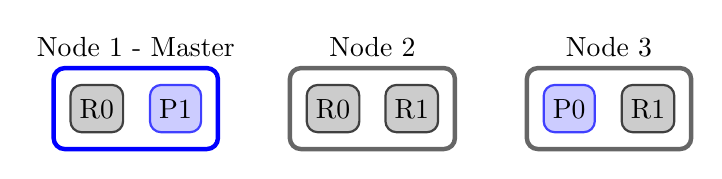
\begin{tikzpicture}
		\tikzstyle{shard}=[thick,draw=blue!75,fill=blue!20,minimum size=6mm, rounded corners]
		\tikzstyle{replica}=[thick,draw=black!75,fill=black!20,minimum size=6mm, rounded corners]
		\tikzstyle{node_master}=[draw=blue, ultra thick, inner sep=2mm, rounded corners]
		\tikzstyle{node}=[node_master, draw=black!60]
		\tikzstyle{node_text}=[draw=none, fill=none, above]

		\begin{scope}
			\node [replica] (R0-1) {R0};
			\node [shard] (P1) [right of=R0-1] {P1};

			\node (node1) [node_master,fit=(R0-1) (P1)] {};
			\node at (node1.north) [node_text] {Node 1 - Master};
		\end{scope}

		\begin{scope}[xshift=30mm]
			\node [replica] (R0-2) {R0};
			\node [replica] (R1-1) [right of=R0-2] {R1};

			\node (node2) [node, fit=(R0-2) (R1-1)] {};
			\node at (node2.north) [node_text] {Node 2};
		\end{scope}

		\begin{scope}[xshift=60mm]
			\node [shard] (P0) {P0};
			\node [replica] (R1-2) [right of=P0] {R1};

			\node (node3) [node, fit=(P0) (R1-2)] {};
			\node at (node3.north) [node_text] {Node 3};
		\end{scope}
	\end{tikzpicture}
	\caption{Simple cluster}
\end{figure}

\paragraph{} We can send our requests to any node in the cluster. Every node is fully capable of serving any request. Every node knows the location of every document in the cluster and so can forward requests directly to the required node. In the examples below, we will send all of our requests to \texttt{Node 1}, which we will refer to as the requesting node.

\paragraph{} When sending requests, it is good practice to round-robin through all the nodes in the cluster, in order to spread the load.

\subsection{PUT and DELETE request (create, index and delete)}

\begin{figure}[h!]
	\centering
	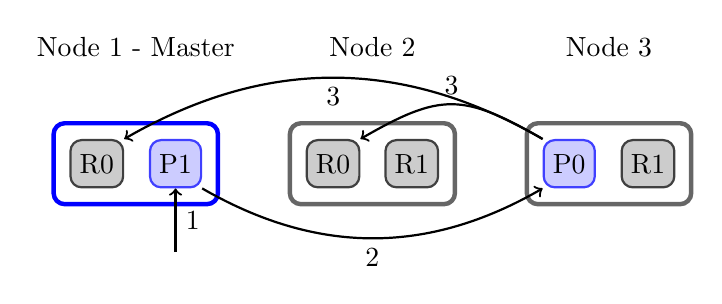
\begin{tikzpicture}
		\tikzstyle{shard}=[thick,draw=blue!75,fill=blue!20,minimum size=6mm, rounded corners]
		\tikzstyle{replica}=[thick,draw=black!75,fill=black!20,minimum size=6mm, rounded corners]
		\tikzstyle{node_master}=[draw=blue, ultra thick, inner sep=2mm, rounded corners]
		\tikzstyle{node}=[node_master, draw=black!60]
		\tikzstyle{node_text}=[draw=none, fill=none, above, yshift=7mm]
		\tikzstyle{arrow}=[thick]

		\begin{scope}
			\node [replica] (R0-1) {R0};
			\node [shard] (P1) [right of=R0-1] {P1};

			\node (node1) [node_master,fit=(R0-1) (P1)] {};
			\node at (node1.north) [node_text] {Node 1 - Master};
		\end{scope}

		\begin{scope}[xshift=30mm]
			\node [replica] (R0-2) {R0};
			\node [replica] (R1-1) [right of=R0-2] {R1};

			\node (node2) [node, fit=(R0-2) (R1-1)] {};
			\node at (node2.north) [node_text] {Node 2};
		\end{scope}

		\begin{scope}[xshift=60mm]
			\node [shard] (P0) {P0};
			\node [replica] (R1-2) [right of=P0] {R1};

			\node (node3) [node, fit=(P0) (R1-2)] {};
			\node at (node3.north) [node_text] {Node 3};
		\end{scope}

	\node (invis1) [below of=P1] {};
	\path[->] (invis1.south) edge [arrow] node [right] {1} (P1);

	\path[->] (P1.south east) edge [arrow, bend right] node [below] {2} (P0.south west);

    \path[->] (P0.north west) edge [arrow, bend right, looseness=1.3] node [above] {3} (R0-2.north east);
    \path[->] (P0.north west) edge [arrow, bend right] node [below] {3} (R0-1.north east);

	\end{tikzpicture}
	\caption{PUT or DELETE request case}
\end{figure}

Below we list the sequence of steps necessary to successfully create, index or delete a document on both the primary and any replica shards:

\begin{enumerate}
	\item The client sends a create, index or delete request to \texttt{Node\_1}.
	\item The node uses the document’s \texttt{\_id} to determine that the document belongs to shard 0. It forwards the request to \texttt{Node 3}, where the primary copy of shard 0 is currently allocated. 
	\item \texttt{Node 3} executes the request on the primary shard. If it is successful, it forwards the request in parallel to the replica shards on \texttt{Node 1} and \texttt{Node 2}. Once all of the replica shards report success, \texttt{Node 3} reports success to the requesting node, which reports success to the client. 
\end{enumerate}

\paragraph{} What happens if insufficient shard copies are available ? Elasticsearch waits, in the hope that more shards will appear. By default it will wait up to one minute. If you need to, you can use the \texttt{timeout} parameter to make it abort sooner: 100 is 100 milliseconds, 30s is 30 seconds.

\subsection{GET request (retrieve)}

\begin{figure}[h!]
	\centering
	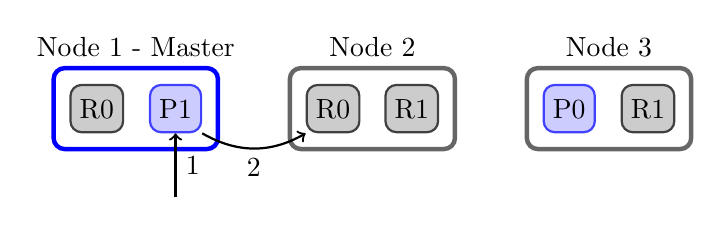
\begin{tikzpicture}
		\tikzstyle{shard}=[thick,draw=blue!75,fill=blue!20,minimum size=6mm, rounded corners]
		\tikzstyle{replica}=[thick,draw=black!75,fill=black!20,minimum size=6mm, rounded corners]
		\tikzstyle{node_master}=[draw=blue, ultra thick, inner sep=2mm, rounded corners]
		\tikzstyle{node}=[node_master, draw=black!60]
		\tikzstyle{node_text}=[draw=none, fill=none, above]
		\tikzstyle{arrow}=[thick]

		\begin{scope}
			\node [replica] (R0-1) {R0};
			\node [shard] (P1) [right of=R0-1] {P1};

			\node (node1) [node_master,fit=(R0-1) (P1)] {};
			\node at (node1.north) [node_text] {Node 1 - Master};
		\end{scope}

		\begin{scope}[xshift=30mm]
			\node [replica] (R0-2) {R0};
			\node [replica] (R1-1) [right of=R0-2] {R1};

			\node (node2) [node, fit=(R0-2) (R1-1)] {};
			\node at (node2.north) [node_text] {Node 2};
		\end{scope}

		\begin{scope}[xshift=60mm]
			\node [shard] (P0) {P0};
			\node [replica] (R1-2) [right of=P0] {R1};

			\node (node3) [node, fit=(P0) (R1-2)] {};
			\node at (node3.north) [node_text] {Node 3};
		\end{scope}

	\node (invis1) [below of=P1] {};
	\path[->] (invis1.south) edge [arrow] node [right] {1} (P1);

	\path[->] (P1.south east) edge [arrow, bend right] node [below] {2} (R0-2.south west);

	\end{tikzpicture}
	\caption{GET request case}
\end{figure}

Below we list the sequence of steps to retrieve a document from either a primary or replica shard:

\begin{enumerate}
	\item The client sends a get request to \texttt{Node 1}.
	\item The node uses the document’s \texttt{\_id} to determine that the document belongs to shard 0. Copies of shard 0 exist on all three nodes. On this occasion, it forwards the request to \texttt{Node 2}, which returns the document. 
\end{enumerate}

\paragraph{} For read requests, the requesting node will choose a different shard copy on every request  --  it round-robins through the nodes.

\paragraph{} It is possible that a document has been indexed on the primary shard but has not yet been copied to the replica shards. In this case a replica might report that the document doesn’t exist, while the primary would have returned the document successfully.

\subsection{Manage primary shard and replica shard}

\paragraph{Important} Before running the following examples you must have a empty one-node cluster that is a single instance of Elasticsearch and no indices.

\paragraph{} Let’s create an index called \texttt{megacorp} in our empty one-node cluster. By default, indices are assigned 5 primary shards, but for the purpose of this demonstration, we’ll assign just 3 primary shards and 1 replica (one replica of every primary shard):

\begin{command}
curl -XPUT 'http://localhost:9200/megacorp' -d '
{
	"settings" : {
		"number_of_shards" : 3,
		"number_of_replicas" : 1
	}
}'
\end{command}

Following this, all 3 primary shards have been allocated to \texttt{Node 1}.

\begin{figure}[h!]
	\centering
	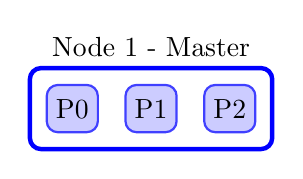
\begin{tikzpicture}
		\tikzstyle{shard}=[thick,draw=blue!75,fill=blue!20,minimum size=6mm, rounded corners]
		\tikzstyle{replica}=[thick,draw=black!75,fill=black!20,minimum size=6mm, rounded corners]
		\tikzstyle{node_master}=[draw=blue, ultra thick, inner sep=2mm, rounded corners]
		\tikzstyle{node}=[node_master, draw=black!60]
		\tikzstyle{node_text}=[draw=none, fill=none, above]

		\begin{scope}
			\node [shard] (P0) {P0};
			\node [shard] (P1) [right of=P0] {P1};
			\node [shard] (P2) [right of=P1] {P2};

			\node (node1) [node_master,fit=(P0) (P1) (P2)] {};
			\node at (node1.north) [node_text] {Node 1 - Master};
		\end{scope}

	\end{tikzpicture}
	\caption{1 node with 3 primary shards}
\end{figure}

Now let's check the cluster status:

\begin{command}
curl -XGET 'http://localhost:9200/_cluster/health?pretty'
\end{command}

\begin{command}
{
	"cluster_name" : "elasticsearch",
	"status" : "yellow",
	"timed_out" : false,
	"number_of_nodes" : 1,
	"number_of_data_nodes" : 1,
	"active_primary_shards" : 3,
	"active_shards" : 3,
	"relocating_shards" : 0,
	"initializing_shards" : 0,
	"unassigned_shards" : 3
}
\end{command}

\paragraph{} A cluster health of yellow means that all \textbf{primary shards} are up and running  --  the cluster is capable of serving any request successfully  --  but not all \textbf{replica shards} are active. In fact all three of our replica shards are currently unassigned  --  they haven’t been allocated to a node. It doesn’t make sense to store copies of the same data on the same node. If we were to lose that node, we would lose all copies of our data.

Currently our cluster is fully functional but at risk of data loss in case of hardware failure.

\subsection{Fault tolerance}

\paragraph{} Running a single node means that you have a single point of failure  --  there is no redundancy. Fortunately all we need to do to protect ourselves from data loss is to start another node. A new node will join the cluster automatically as long as it has the same cluster name set in its config file, and it can talk to the other nodes.

\begin{figure}[h!]
	\centering
	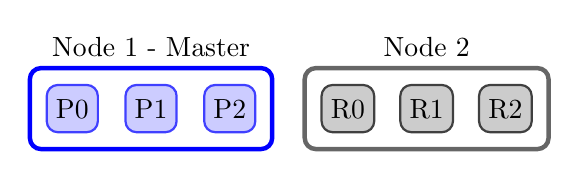
\begin{tikzpicture}
		\tikzstyle{shard}=[thick,draw=blue!75,fill=blue!20,minimum size=6mm, rounded corners]
		\tikzstyle{replica}=[thick,draw=black!75,fill=black!20,minimum size=6mm, rounded corners]
		\tikzstyle{node_master}=[draw=blue, ultra thick, inner sep=2mm, rounded corners]
		\tikzstyle{node}=[node_master, draw=black!60]
		\tikzstyle{node_text}=[draw=none, fill=none, above]

		\begin{scope}
			\node [shard] (P0) {P0};
			\node [shard] (P1) [right of=P0] {P1};
			\node [shard] (P2) [right of=P1] {P2};

			\node (node1) [node_master,fit=(P0) (P1) (P2)] {};
			\node at (node1.north) [node_text] {Node 1 - Master};
		\end{scope}

		\begin{scope}[xshift=35mm]
			\node [replica] (R0) {R0};
			\node [replica] (R1) [right of=R0] {R1};
			\node [replica] (R2) [right of=R1] {R2};

			\node (node2) [node,fit=(R0) (R1) (R2)] {};
			\node at (node2.north) [node_text] {Node 2};
		\end{scope}

	\end{tikzpicture}
	\caption{2 nodes with 3 primary shards and 1 replica shard for each primary shard}
\end{figure}

\paragraph{} The second node has joined the cluster and three replica shards have been allocated to it  --  one for each primary shard. That means that we can lose either node and all of our data will be intact.

\paragraph{} Any newly indexed document will first be stored on a primary shard, then copied in parallel to the associated replica shard(s). This ensures that our document can be retrieved from a primary shard or from any of its replicas.

\paragraph{} Wait few seconds and check the cluster status:

\begin{command}
curl -XGET 'http://localhost:9200/_cluster/health?pretty'
\end{command}

\begin{command}
{
	"cluster_name" : "elasticsearch",
	"status" : "green",
	"timed_out" : false,
	"number_of_nodes" : 2,
	"number_of_data_nodes" : 2,
	"active_primary_shards" : 3,
	"active_shards" : 6,
	"relocating_shards" : 0,
	"initializing_shards" : 0,
	"unassigned_shards" : 0
}
\end{command}

Our cluster is not only fully functional but also always available.

\subsection{Improve performance with horizontal scaling}

\paragraph{} The only thing you have to do is to start another instance of Elasticsearch with the same \texttt{cluster.name} and Elasticsearch will automatically spread the load.

If we add a third node (instance of Elasticsearch), the cluster looks like:

\begin{figure}[h!]
	\centering
	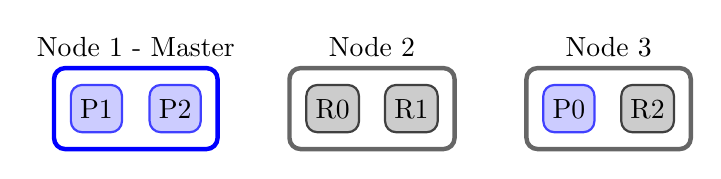
\begin{tikzpicture}
		\tikzstyle{shard}=[thick,draw=blue!75,fill=blue!20,minimum size=6mm, rounded corners]
		\tikzstyle{replica}=[thick,draw=black!75,fill=black!20,minimum size=6mm, rounded corners]
		\tikzstyle{node_master}=[draw=blue, ultra thick, inner sep=2mm, rounded corners]
		\tikzstyle{node}=[node_master, draw=black!60]
		\tikzstyle{node_text}=[draw=none, fill=none, above]

		\begin{scope}
			\node [shard] (P1) {P1};
			\node [shard] (P2) [right of=P1] {P2};

			\node (node1) [node_master,fit=(P1) (P2)] {};
			\node at (node1.north) [node_text] {Node 1 - Master};
		\end{scope}

		\begin{scope}[xshift=30mm]
			\node [replica] (R0) {R0};
			\node [replica] (R1) [right of=R0] {R1};

			\node (node2) [node,fit=(R0) (R1)] {};
			\node at (node2.north) [node_text] {Node 2};
		\end{scope}

		\begin{scope}[xshift=60mm]
			\node [shard] (P0) {P0};
			\node [replica] (R2) [right of=P0] {R2};

			\node (node3) [node,fit=(P0) (R2)] {};
			\node at (node3.north) [node_text] {Node 3};
		\end{scope}

	\end{tikzpicture}
	\caption{3 nodes with 3 primary shards and 1 replica shard for each primary shard}
\end{figure}

\paragraph{} One shard each from \texttt{Node 1} and \texttt{Node 2} have moved to the new \texttt{Node 3} and we have two shards per node, instead of three. This means that the hardware resources (CPU, RAM, I/O) of each node are being shared between fewer shards, allowing each shard to perform better.

\paragraph{} A shard is a fully fledged search engine in its own right, and is capable of using all of the resources of a single node. With our total of 6 shards (3 primaries and 3 replicas) our index is capable of scaling out to a maximum of 6 nodes, with one shard on each node and each shard having access to 100\% of its node’s resources.

\paragraph{} But what if we want to scale our search to more than 6 nodes ?

\paragraph{} The number of primary shards is fixed at the moment an index is created. Effectively, that number defines the maximum amount of data that can be stored in the index. (The actual number depends on your data, your hardware and your use case). However, read requests  --  searches or document retrieval  --  can be handled by a primary or a replica shard, so the more copies of data that you have, the more search throughput we can handle.

\paragraph{} The number of replica shards can be changed dynamically on a live cluster, allowing us to scale up or down as demand requires. Let’s increase the number of replicas from 1 to 2:

\begin{command}
curl -XPUT 'http://localhost:9200/megacorp/_settings' -d '
{
   "number_of_replicas" : 2
}'
\end{command}

Now the cluster looks like:

\begin{figure}[h!]
	\centering
	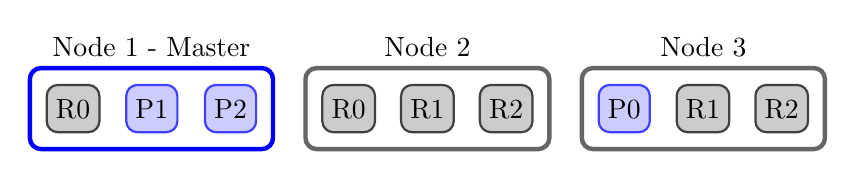
\begin{tikzpicture}
		\tikzstyle{shard}=[thick,draw=blue!75,fill=blue!20,minimum size=6mm, rounded corners]
		\tikzstyle{replica}=[thick,draw=black!75,fill=black!20,minimum size=6mm, rounded corners]
		\tikzstyle{node_master}=[draw=blue, ultra thick, inner sep=2mm, rounded corners]
		\tikzstyle{node}=[node_master, draw=black!60]
		\tikzstyle{node_text}=[draw=none, fill=none, above]

		\begin{scope}
			\node [replica] (R0) {R0};
			\node [shard] (P1) [right of=R0] {P1};
			\node [shard] (P2) [right of=P1] {P2};

			\node (node1) [node_master,fit=(R0) (P1) (P2)] {};
			\node at (node1.north) [node_text] {Node 1 - Master};
		\end{scope}

		\begin{scope}[xshift=35mm]
			\node [replica] (R0) {R0};
			\node [replica] (R1) [right of=R0] {R1};
			\node [replica] (R2) [right of=R1] {R2};

			\node (node2) [node,fit=(R0) (R1) (R2)] {};
			\node at (node2.north) [node_text] {Node 2};
		\end{scope}

		\begin{scope}[xshift=70mm]
			\node [shard] (P0) {P0};
			\node [replica] (R1) [right of=P0] {R1};
			\node [replica] (R2) [right of=R1] {R2};

			\node (node3) [node,fit=(P0) (R1) (R2)] {};
			\node at (node3.north) [node_text] {Node 3};
		\end{scope}

	\end{tikzpicture}
	\caption{3 nodes with 3 primary shards and 2 replica shards for each primary shard}
\end{figure}

\subsection{Failure case}

\paragraph{} At this point, the cluster can loose 2 nodes without data lost so let's check.

\paragraph{} Cluster after killing ths first node (master node):

\begin{figure}[h!]
	\centering
	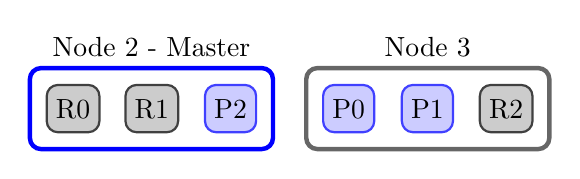
\begin{tikzpicture}
		\tikzstyle{shard}=[thick,draw=blue!75,fill=blue!20,minimum size=6mm, rounded corners]
		\tikzstyle{replica}=[thick,draw=black!75,fill=black!20,minimum size=6mm, rounded corners]
		\tikzstyle{node_master}=[draw=blue, ultra thick, inner sep=2mm, rounded corners]
		\tikzstyle{node}=[node_master, draw=black!60]
		\tikzstyle{node_text}=[draw=none, fill=none, above]

		\begin{scope}[xshift=35mm]
			\node [replica] (R0) {R0};
			\node [replica] (R1) [right of=R0] {R1};
			\node [shard] (P2) [right of=R1] {P2};

			\node (node2) [node_master,fit=(R0) (R1) (P2)] {};
			\node at (node2.north) [node_text] {Node 2 - Master};
		\end{scope}

		\begin{scope}[xshift=70mm]
			\node [shard] (P0) {P0};
			\node [shard] (P1) [right of=P0] {P1};
			\node [replica] (R2) [right of=P1] {R2};

			\node (node3) [node,fit=(P0) (P1) (R2)] {};
			\node at (node3.north) [node_text] {Node 3};
		\end{scope}

	\end{tikzpicture}
	\caption{Cluster after killing the first node}
\end{figure}

\paragraph{} The node we killed was the master node. A cluster must have a master node in order to function correctly, so the first thing that happened was that the nodes elected a new master: \texttt{Node 2}.

\paragraph{} Primary shards 1 and 2 were lost when we killed \texttt{Node 1} and our index cannot function properly if it is missing primary shards. If we had checked the cluster health at this point, we would have seen status \texttt{red}: not all primary shards are active !

\paragraph{} Fortunately a complete copy of the two lost primary shards exists on other nodes, so the first thing that the new master node did was to promote the replicas of these shards on \texttt{Node 2} and \texttt{Node 3} to be primaries, putting us back into cluster health \texttt{yellow}. This promotion process was instantaneous, like the flick of a switch.

\paragraph{} So why is our cluster health \texttt{yellow} and not \texttt{green} ? We have all 3 primary shards, but we specified that we wanted two replicas of each primary and currently only one replica is assigned. This prevents us from reaching \texttt{green}, but we’re not too worried here: were we to kill \texttt{Node 2} as well, our application could still keep running without data loss because \texttt{Node 3} contains a copy of every shard.

\subsection{Discovery}

\paragraph{} The discovery module is responsible for discovering nodes within a cluster, as well as electing a master node.

\paragraph{Note} Elasticsearch is a peer to peer based system, nodes communicate with one another directly if operations are delegated / broadcast. All the main APIs (index, delete, search) do not communicate with the master node. The responsibility of the master node is to maintain the global cluster state, and act if nodes join or leave the cluster by reassigning shards. Each time a cluster state is changed, the state is made known to the other nodes in the cluster (the manner depends on the actual discovery implementation).

\subsubsection{Settings}

The \texttt{cluster.name} allows to create separated clusters from one another. The default value for the cluster name is "elasticsearch", though it is recommended to change this to reflect the logical group name of the cluster running.

\subsubsection{Discovery type}

\begin{itemize}
	\item Azure discovery
	\item EC2 discovery
	\item Google compure engine discovery
	\item Zen discovery (builtin and default)
\end{itemize}

\subsubsection{Zen discovery}

\paragraph{} The zen discovery is the built in discovery module for elasticsearch and the default. It provides both multicast and unicast discovery as well being easily extended to support cloud environments.

\paragraph{ping} This is the process where a node uses the discovery mechanisms to find other nodes. There is support for both multicast and unicast based discovery (can be used in conjunction as well).

\paragraph{multicast} Multicast ping discovery of other nodes is done by sending one or more multicast requests where existing nodes that exists will receive and respond to. It provides the following settings with the \texttt{discovery.zen.ping.multicast} prefix:

\begin{itemize}
	\item group : the group address to use. Defaults to \texttt{224.2.2.4}.
	\item port : the port to use. Defaults to \texttt{54328}.
	\item ttl : the ttl of the multicast message. Defaults to 3.
	\item address : the address to bind to, defaults to null which means it will bind to all available network interfaces.
	\item enabled : whether multicast ping discovery is enabled. Defaults to true.
\end{itemize}

\paragraph{unicast} The unicast discovery allows to perform the discovery when multicast is not enabled. It basically requires a list of hosts to use that will act as gossip routers. It provides the following settings with the \texttt{discovery.zen.ping.unicast} prefix:

\begin{itemize}
	\item hosts : Either an array setting or a comma delimited setting. Each value is either in the form of \texttt{host:port}, or in the form of \texttt{host[port1-port2]}.
\end{itemize}

%%%%%%%%%%%%%%%%%%%%%%%%%%%%%%%%%%%%%%%%%%%%%%%%%%%%%%%%%%%%%%%%%%%%%%%%%%%%%%%%%%%%%%%%%%%%%%%%%%%%%%%%%%%%%%%%%%%%%%%%
%%%%%%%%%%%%%%%%%%%%%%%%%%%%%%%%%%%%%%%%%%%    Plug it with MongoDB    %%%%%%%%%%%%%%%%%%%%%%%%%%%%%%%%%%%%%%%%%%%%%%%%%
%%%%%%%%%%%%%%%%%%%%%%%%%%%%%%%%%%%%%%%%%%%%%%%%%%%%%%%%%%%%%%%%%%%%%%%%%%%%%%%%%%%%%%%%%%%%%%%%%%%%%%%%%%%%%%%%%%%%%%%%
\section{Plug it with MongoDB}


\subsection{Prerequisites}

The plugin has a dependency to elasticsearch-mapper-attachment.

\paragraph{} To install it, simply run:

\begin{command}
./bin/plugin -install elasticsearch/elasticsearch-mapper-attachments/2.0.0
\end{command}

\paragraph{} Then install the river plugin:

\begin{command}
./bin/plugin --install com.github.richardwilly98.elasticsearch/elasticsearch-river-mongodb/2.0.0
\end{command}

\subsection{Setup river plugin}

\paragraph{} Create a new river for each MongoDB collection that should be indexed by ElasticSearch.

\begin{itemize}
	\item Replace \$\{es.river.name\}, \$\{mongo.db.name\}, \$\{mongo.collection.name\}, \\\$\{mongo.is.gridfs.collection\}, \$\{es.index.name\} and \$\{es.type.name\} by the correct values. Parameters servers, options and credentials are optional.
	\begin{itemize}
		\item \$\{es.river.name\} is the Elasticsearch river name
		\item servers is an array of mongo instances. If not specify the \$\{mongo.instance1.host\} (default value: localhost) and \$\{mongo.instance1.port\} (default value: 27017)
		\item options define additional river options.
		\begin{itemize}
			\item Mongo options settings used by the driver (only secondary\_read\_preference is implemented).
			\item \textbf{drop\_collection} can be used to remove all document associated with the index type when the collection is dropped from MongotDB.
			\item \textbf{exclude\_fields} this option will remove unwanted fields from MongoDB before documents are indexed in ES.
			\item \textbf{include\_fields} this option will only include specified fields from MongoDB before documents are indexed in ES. This option is tmutually exclusive with exclude\_fields.
			\item \textbf{include\_collection} this option will include the collection name in the document indexed \$\{mongo.include.collection\} is the tattribute name.
			\item \textbf{import\_all\_collections} this option will import all collections of the specified database. \$\{mongo.collection.name\} value its ignored in that scenario.
			\item \textbf{initial\_timestamp} this option set the timestamp for the initial document import.
			\item \textbf{skip\_initial\_import} this option will skip the initial import (using collection data) and directly use oplog.rs collectiont. The default is false.
			\item \textbf{store\_statistics} statistics of documents indexed will be store in ES in \\\_river/\$\{es.river.name\}
		\end{itemize}
		\item \textbf{credentials} is an array of the credential required by the databases. db can be ‘admin’ or ‘local’. The credentials are used to connect to local and \$\{mongo.db.name\}.
		\item Deprecated use bulk processor settings – In index a throttle size can be defined \$\{es.throttle.size\} default value is 500.
		\item Deprecated use bulk processor settings – In index a bulk update size can be defined \$\{es.bulk.size\} default value is 100.
		\item In index bulk processor settings can be changed: \$\{es.bulk.actions\} default value is 1000, \$\{es.bulk.size\} default value is 5mb, \$\{es.bulk.concurrent.requests\} default value is 50, \$\{es.bulk.flush.interval\} default value is 10ms.
	\end{itemize}
	\item In mongo a custom filter can be added in \$\{mongo.filter\}.
\end{itemize}

\begin{command}
curl -XPUT "localhost:9200/_river/${es.river.name}/_meta" -d '
{
	"type": "mongodb",
	"mongodb": {
		"servers": [
			{ "host": ${mongo.instance1.host}, "port": ${mongo.instance1.port} },
			{ "host": ${mongo.instance2.host}, "port": ${mongo.instance2.port} }
		],
		"options": {
			"secondary_read_preference" : true,
			"drop_collection": ${mongo.drop.collection},
			"exclude_fields": ${mongo.exclude.fields},
			"include_fields": ${mongo.include.fields},
			"include_collection": ${mongo.include.collection},
			"import_all_collections": ${mongo.import.all.collections},
			"initial_timestamp": {
				"script_type": ${mongo.initial.timestamp.script.type},
				"script": ${mongo.initial.timestamp.script}
			},
			"skip_initial_import" : ${mongo.skip.initial.import},
			"store_statistics" : ${mongo.store.statistics},
		},
		"credentials": [
			{ "db": "local", "user": ${mongo.local.user}, "password": ${mongo.local.password} },
			{ "db": "admin", "user": ${mongo.db.user}, "password": ${mongo.db.password} }
		],
		"db": ${mongo.db.name},
		"collection": ${mongo.collection.name},
		"gridfs": ${mongo.is.gridfs.collection},
		"filter": ${mongo.filter}
	},
	"index": {
		"name": ${es.index.name},
		"throttle_size": ${es.throttle.size},
		"bulk_size": ${es.bulk.size},
		"type": ${es.type.name}
		"bulk": {
			"actions": ${es.bulk.actions},
			"size": ${es.bulk.size},
			"concurrent_requests": ${es.bulk.concurrent.requests},
			"flush_interval": ${es.bulk.flush.interval}
		}
	}
}'
\end{command}

\end{document}%

